% answers.tex —— 2013 年·北京卷·文科 · 参考答案与详细解析片段
% 由 tools/generate_projects.py 依来源总账自 2013/2013_数学真题_北京文_试题.md + 2013/2013_数学真题_北京文_解析正文.md + 2013/2013_数学真题_北京文_答案要点.md 生成，勿手改（改源 MD 后重跑）


\begin{answer}
\gksolhead{1}{}

\textbf{题目}：

已知集合 $A=\{-1,0,1\}$，$B=\{x\mid-1\leqslant x<1\}$，则 $A\cap B=$\mbox{（　　）}

（A）$\{0\}$；（B）$\{-1,0\}$；（C）$\{0,1\}$；（D）$\{-1,0,1\}$。

\Needspace{4\baselineskip}
\textbf{解析}
\Needspace{5\baselineskip}
集合 $B$ 由满足 $-1\leqslant x<1$ 的实数组成。逐个数检验 $A$ 中的元素：
\nopagebreak[4]
\[-1\in B,\qquad 0\in B,\qquad 1\notin B\ (\text{\text{因为} }1<1\text{ \text{不成立}}).\]
\Needspace{5\baselineskip}
所以
\nopagebreak[4]
\[A\cap B=\{-1,0\}.\]
选 B。

\gkanswer{答案：B。$-1$，$0$ 在 $B$ 中而 $1\notin B$，故 $A\cap B=\{-1,0\}$。}

\end{answer}
\begin{answer}
\gksolhead{2}{}

\textbf{题目}：

设 $a$，$b$，$c\in\mathbf R$，且 $a>b$，则\mbox{（　　）}

（A）$ac>bc$；（B）$\dfrac1a<\dfrac1b$；（C）$a^2>b^2$；（D）$a^3>b^3$。

\Needspace{4\baselineskip}
\textbf{解析}
逐项判断。取 $c=0$ 得 $ac=bc=0$，故（A）不成立；取 $a=1$，$b=-1$，则 $\dfrac1a=1$，$\dfrac1b=-1$，$\dfrac1a>\dfrac1b$，故（B）不成立；取 $a=1$，$b=-2$，则 $a^2=1<b^2=4$，故（C）不成立。

对（D），$y=x^3$ 在 $\mathbf R$ 上单调递增，故 $a>b$ 必有 $a^3>b^3$。选 D。

\gkanswer{答案：D。$y=x^3$ 在 $\mathbf R$ 上单调递增，故 $a>b$ 时 $a^3>b^3$ 必成立。}

\end{answer}
\begin{answer}
\gksolhead{3}{}

\textbf{题目}：

下列函数中，既是偶函数又在区间 $(0,+\infty)$ 上单调递减的是\mbox{（　　）}

（A）$y=\dfrac1x$；（B）$y=\mathrm e^{-x}$；（C）$y=-x^2+1$；（D）$y=\lg|x|$。

\Needspace{4\baselineskip}
\textbf{解析}
逐项检验偶性与单调性：

（A）$y=\dfrac1x$ 是奇函数，排除；

（B）$y=\mathrm e^{-x}$ 满足 $f(-x)=\mathrm e^{x}\neq f(x)$，不是偶函数，排除；

（C）$y=-x^2+1$ 满足 $f(-x)=-x^2+1=f(x)$，是偶函数；当 $x\in(0,+\infty)$ 时 $x$ 增大则 $x^2$ 增大、$-x^2+1$ 减小，故在 $(0,+\infty)$ 上单调递减，符合；

（D）$y=\lg|x|$ 是偶函数，但当 $x$ 由 $1$ 增大到 $2$ 时函数值由 $0$ 增大到 $\lg2$，在 $(0,+\infty)$ 上单调递增，排除。

选 C。

\gkanswer{答案：C。$y=-x^2+1$ 是偶函数，且在 $(0,+\infty)$ 上随 $x$ 增大而减小。}

\end{answer}
\begin{answer}
\gksolhead{4}{}

\textbf{题目}：

在复平面内，复数 $\mathrm i(2-\mathrm i)$ 对应的点位于\mbox{（　　）}

（A）第一象限；（B）第二象限；（C）第三象限；（D）第四象限。

\Needspace{4\baselineskip}
\textbf{解析}
\Needspace{5\baselineskip}
由复数乘法，
\nopagebreak[4]
\[\mathrm i(2-\mathrm i)=2\mathrm i-\mathrm i^2=2\mathrm i+1=1+2\mathrm i.\]
实部为 $1>0$，虚部为 $2>0$，故对应点 $(1,2)$ 位于第一象限。选 A。

\gkanswer{答案：A。$\mathrm i(2-\mathrm i)=1+2\mathrm i$，实部、虚部均为正，对应点在第一象限。}

\end{answer}
\begin{answer}
\gksolhead{5}{}

\textbf{题目}：

在 $\triangle ABC$ 中，$a=3$，$b=5$，$\sin A=\dfrac13$，则 $\sin B=$\mbox{（　　）}

（A）$\dfrac15$；（B）$\dfrac59$；（C）$\dfrac{\sqrt5}3$；（D）$1$。

\Needspace{4\baselineskip}
\textbf{解析}
\Needspace{5\baselineskip}
由正弦定理，
\nopagebreak[4]
\[\frac{a}{\sin A}=\frac{b}{\sin B},\]
\Needspace{5\baselineskip}
所以
\nopagebreak[4]
\[\sin B=\frac{b\sin A}{a}=\frac{5\cdot\dfrac13}{3}=\frac59.\]
选 B。

\gkanswer{答案：B。由正弦定理 $\sin B=\dfrac{b\sin A}a=\dfrac53\times\dfrac13=\dfrac59$。}

\end{answer}
\begin{answer}
\gksolhead{6}{}

\textbf{题目}：

执行如图所示的程序框图，输出的 $S$ 值为\mbox{（　　）}
\nopagebreak[4]
\begin{center}% 2013 年北京卷文科第 6 题：程序框图。
% 来源 PDF：普通高考/2013/2013北京文.pdf，第 1 页（印面 789）左栏。
% 流程：开始 → i=0,S=1 → S=(S^2+1)/(2S+1) → i=i+1 → i≥2?
%       是：输出 S → 结束；否：向右引出后回到 S 赋值框上方。
\begin{tikzpicture}[font=\footnotesize, >=Stealth, line width=0.45pt,
  term/.style={draw, rounded corners=6pt, minimum height=1.8em, inner xsep=9pt},
  io/.style={draw, trapezium, trapezium left angle=70, trapezium right angle=110,
             minimum height=1.8em, inner xsep=6pt},
  box/.style={draw, minimum height=1.9em, inner xsep=6pt},
  dec/.style={draw, diamond, aspect=2.4, inner sep=1pt}]
  \node[term] (start) at (0,0) {开始};
  \node[box] (init) at (0,-1.05) {$i=0$，$S=1$};
  \node[box] (assign) at (0,-2.35) {$S=\dfrac{S^2+1}{2S+1}$};
  \node[box] (inc) at (0,-3.70) {$i=i+1$};
  \node[dec] (cond) at (0,-5.05) {$i\geqslant2$};
  \node[io] (out) at (0,-6.40) {输出 $S$};
  \node[term] (end) at (0,-7.50) {结束};
  \draw[->] (start) -- (init);
  \draw[->] (init) -- (assign);
  \draw[->] (assign) -- (inc);
  \draw[->] (inc) -- (cond);
  \draw[->] (cond) -- node[right] {是} (out);
  \draw[->] (out) -- (end);
  % 循环支路：从判断框右侧引出，上行后折回 S 赋值框顶边
  \coordinate (r1) at ($(cond.east)+(2.3,0)$);
  \coordinate (up) at ($(assign.north)+(0,0.45)$);
  \draw (cond.east) -- node[above] {否} (r1) -- (r1 |- up) -- (0.55,0 |- up);
  \draw[->] (0.55,0 |- up) -- (0.55,0 |- assign.north);
\end{tikzpicture}
\end{center}
\nopagebreak[4]
（A）$1$；（B）$\dfrac23$；（C）$\dfrac{13}{21}$；（D）$\dfrac{610}{987}$。

\Needspace{4\baselineskip}
\textbf{解析}
初始 $i=0$，$S=1$。

\Needspace{5\baselineskip}
第一次执行循环体：
\nopagebreak[4]
\[S=\frac{1^2+1}{2\times1+1}=\frac23,\qquad i=1.\]
判断 $i\geqslant2$：因为 $1\geqslant2$ 不成立，返回循环体。

\Needspace{5\baselineskip}
第二次执行循环体：
\nopagebreak[4]
\[S=\frac{\left(\dfrac23\right)^2+1}{2\cdot\dfrac23+1}
=\frac{\dfrac49+1}{\dfrac43+1}
=\frac{\dfrac{13}9}{\dfrac73}
=\frac{13}9\cdot\frac37=\frac{13}{21},\qquad i=2.\]
\Needspace{5\baselineskip}
判断 $i\geqslant2$：因为 $2\geqslant2$ 成立，输出
\nopagebreak[4]
\[S=\frac{13}{21}.\]
选 C。

\gkanswer{答案：C。循环两次后 $S=\dfrac{13}{21}$ 且 $i=2\geqslant2$，故输出 $\dfrac{13}{21}$。}

\end{answer}
\begin{answer}
\gksolhead{7}{}

\textbf{题目}：

双曲线 $x^2-\dfrac{y^2}m=1$ 的离心率大于 $\sqrt2$ 的充分必要条件是\mbox{（　　）}

（A）$m>\dfrac12$；（B）$m\geqslant1$；（C）$m>1$；（D）$m>2$。

\Needspace{4\baselineskip}
\textbf{解析}
\Needspace{5\baselineskip}
方程 $x^2-\dfrac{y^2}m=1$ 表示双曲线时 $m>0$，此时 $a^2=1$，$b^2=m$，故
\nopagebreak[4]
\[c^2=a^2+b^2=1+m,\qquad e^2=\frac{c^2}{a^2}=1+m.\]
\Needspace{5\baselineskip}
离心率大于 $\sqrt2$ 等价于
\nopagebreak[4]
\[e^2>2\iff1+m>2\iff m>1.\]
因此充分必要条件是 $m>1$。选 C。

\gkanswer{答案：C。$e^2=1+m>2$ 即 $m>1$（$m>0$ 已由方程表示双曲线保证）。}

\end{answer}
\begin{answer}
\gksolhead{8}{}

\textbf{题目}：

如图，在正方体 $ABCD-A_1B_1C_1D_1$ 中，$P$ 为对角线 $BD_1$ 的三等分点，$P$ 到各顶点的距离的不同取值有\mbox{（　　）}
\nopagebreak[4]
\begin{center}% 2013 年北京卷文科第 8 题：正方体 ABCD-A1B1C1D1 与对角线 BD1 的三等分点 P。
% 来源 PDF：普通高考/2013/2013北京文.pdf，第 1 页（印面 789）中栏上方。
% 可见棱用实线，被遮住的 PA 类棱用虚线；BD1 为点划线，P 为其三等分点。
\begin{tikzpicture}[font=\footnotesize, line width=0.45pt]
  \coordinate (A)  at (0,0);
  \coordinate (B)  at (3,0);
  \coordinate (C)  at (4.3,1.3);
  \coordinate (D)  at (1.3,1.3);
  \coordinate (A1) at (0,3);
  \coordinate (B1) at (3,3);
  \coordinate (C1) at (4.3,4.3);
  \coordinate (D1) at (1.3,4.3);
  % 可见棱
  \draw (A) -- (B) -- (C) -- (C1) -- (B1) -- (B);
  \draw (A1) -- (B1) -- (C1) -- (D1) -- cycle;
  \draw (A1) -- (A);
  % 被遮挡的棱
  \draw[dashed] (A) -- (D) -- (C);
  \draw[dashed] (D) -- (D1);
  % 对角线 BD1 与三等分点 P
  \draw[densely dotted] (B) -- (D1);
  \coordinate (P) at ($(B)!0.3333!(D1)$);
  \fill (P) circle (1.5pt);
  \node[right] at (P) {$P$};
  % 顶点标注
  \node[below left]  at (A)  {$A$};
  \node[below right] at (B)  {$B$};
  \node[right]       at (C)  {$C$};
  \node[above left]  at (D)  {$D$};
  \node[left]        at (A1) {$A_1$};
  \node[right]       at (B1) {$B_1$};
  \node[right]       at (C1) {$C_1$};
  \node[above left]  at (D1) {$D_1$};
\end{tikzpicture}
\end{center}
\nopagebreak[4]
（A）$3$ 个；（B）$4$ 个；（C）$5$ 个；（D）$6$ 个。

\Needspace{4\baselineskip}
\textbf{解析}
\Needspace{5\baselineskip}
设正方体棱长为 $1$，建立空间直角坐标系：
\nopagebreak[4]
\[A(0,0,0),\ B(1,0,0),\ C(1,1,0),\ D(0,1,0),\]
\nopagebreak[4]
\[A_1(0,0,1),\ B_1(1,0,1),\ C_1(1,1,1),\ D_1(0,1,1).\]
\Needspace{5\baselineskip}
对角线 $BD_1$ 的三等分点可写成
\nopagebreak[4]
\[P=B+t(\overrightarrow{BD_1})=\left(1-t,\ t,\ t\right),\qquad t=\frac13\ \text{\text{或}}\ t=\frac23.\]
\Needspace{5\baselineskip}
取 $t=\dfrac13$，即 $P\left(\dfrac23,\dfrac13,\dfrac13\right)$，逐个计算距离的平方：
\nopagebreak[4]
\[PB^2=\frac19+\frac19+\frac19=\frac13,\qquad PD_1^2=\frac49+\frac49+\frac49=\frac43,\]
\nopagebreak[4]
\[PA^2=\frac49+\frac19+\frac19=\frac23,\qquad PC^2=\frac19+\frac49+\frac19=\frac23,\qquad PB_1^2=\frac19+\frac19+\frac49=\frac23,\]
\nopagebreak[4]
\[PA_1^2=\frac49+\frac19+\frac49=1,\qquad PC_1^2=\frac19+\frac49+\frac49=1,\qquad PD^2=\frac49+\frac49+\frac19=1.\]
\Needspace{5\baselineskip}
故 $P$ 到八个顶点的距离的平方只取 $\dfrac13$，$\dfrac23$，$1$，$\dfrac43$ 四个值，即距离只取
\nopagebreak[4]
\[\frac{\sqrt3}3,\quad\frac{\sqrt6}3,\quad1,\quad\frac{2\sqrt3}3\]
四个不同值。若取 $t=\dfrac23$，注意正方体的对称变换 $(x,y,z)\mapsto(1-x,1-z,1-y)$ 把 $B$ 映为 $D_1$、把 $t=\dfrac13$ 的三等分点映为 $t=\dfrac23$ 的三等分点，且保持所有距离，故不同取值仍为 $4$ 个。选 B。

\gkanswer{答案：B。设棱长为 $1$，$P$ 到八个顶点的距离平方只取 $\dfrac13$，$\dfrac23$，$1$，$\dfrac43$ 四个值。}

\end{answer}
\begin{answer}
\gksolhead{9}{}

\textbf{题目}：

若抛物线 $y^2=2px$ 的焦点坐标为 $(1,0)$，则 $p=$\gkblank{}；准线方程为\gkblank{}。

\Needspace{4\baselineskip}
\textbf{解析}
\Needspace{5\baselineskip}
抛物线 $y^2=2px$ 的焦点为 $\left(\dfrac p2,0\right)$，由题意 $\dfrac p2=1$，故
\nopagebreak[4]
\[p=2.\]
\Needspace{5\baselineskip}
准线方程为
\nopagebreak[4]
\[x=-\frac p2=-1.\]
答案：$p=2$，准线方程为 $x=-1$。

\gkanswer{答案：$p=2$，准线方程为 $x=-1$。由 $\dfrac p2=1$ 得 $p=2$，准线 $x=-\dfrac p2$。}

\end{answer}
\begin{answer}
\gksolhead{10}{}

\textbf{题目}：

某四棱锥的三视图如图所示，该四棱锥的体积为\gkblank{}。
\nopagebreak[4]
\begin{center}% 2013 年北京卷文科第 10 题：四棱锥的三视图。
% 来源 PDF：普通高考/2013/2013北京文.pdf，第 1 页（印面 789）中栏。
% 正视图底边 2+1=3、高 1；侧视图底边 1+2=3、高 1；俯视图为边长 3 的正方形，
% 内部四条线汇聚于顶点的投影（距左边 2、距上边 1）。
\begin{tikzpicture}[font=\footnotesize, line width=0.45pt, >=Stealth]
  % 正（主）视图
  \draw (0,0) -- (3,0) -- (2,1) -- cycle;
  \draw[|<->|] (0,-0.30) -- (1.95,-0.30) node[midway,below] {$2$};
  \draw[|<->|] (2.05,-0.30) -- (3,-0.30) node[midway,below] {$1$};
  \foreach \x in {0,2,3} \draw (\x,-0.18) -- (\x,-0.42);
  \node at (1.5,-1.0) {正（主）视图};
  % 高 1（正视图与侧视图之间）
  \draw[gray!70] (2,1) -- (3.55,1);
  \draw[gray!70] (3,0) -- (3.55,0);
  \draw[|<->|] (3.42,0) -- (3.42,1) node[midway,left] {$1$};
  % 侧（左）视图
  \draw (4.5,0) -- (7.5,0) -- (5.5,1) -- cycle;
  \draw[|<->|] (4.5,-0.30) -- (5.45,-0.30) node[midway,below] {$1$};
  \draw[|<->|] (5.55,-0.30) -- (7.5,-0.30) node[midway,below] {$2$};
  \foreach \x in {4.5,5.5,7.5} \draw (\x,-0.18) -- (\x,-0.42);
  \node at (6.0,-1.0) {侧（左）视图};
  % 俯视图
  \draw (1.2,-1.7) rectangle (4.2,-4.7);
  \coordinate (Q) at (3.2,-2.7);
  \draw (1.2,-1.7) -- (Q);
  \draw (4.2,-1.7) -- (Q);
  \draw (1.2,-4.7) -- (Q);
  \draw (4.2,-4.7) -- (Q);
  \node at (2.7,-5.15) {俯视图};
\end{tikzpicture}
\end{center}
\nopagebreak[4]
\Needspace{4\baselineskip}
\textbf{解析}
\Needspace{5\baselineskip}
由正（主）视图知底面沿左右方向的边长为
\nopagebreak[4]
\[2+1=3,\]
\Needspace{5\baselineskip}
由侧（左）视图知底面沿前后方向的边长为
\nopagebreak[4]
\[1+2=3,\]
\Needspace{5\baselineskip}
俯视图是边长 $3$ 的正方形，与上述两个尺寸一致，故底面是边长为 $3$ 的正方形，面积
\nopagebreak[4]
\[S=3\times3=9.\]
\Needspace{5\baselineskip}
正视图、侧视图的高度均为 $1$，即棱锥的高
\nopagebreak[4]
\[h=1.\]
\Needspace{5\baselineskip}
所以体积
\nopagebreak[4]
\[V=\frac13Sh=\frac13\times9\times1=3.\]
答案：$3$。

\gkanswer{答案：$3$。底面是边长 $3$ 的正方形，高为 $1$，故 $V=\dfrac13\times3\times3\times1=3$。}

\end{answer}
\begin{answer}
\gksolhead{11}{}

\textbf{题目}：

若等比数列 $\{a_n\}$ 满足 $a_2+a_4=20$，$a_3+a_5=40$，则公比 $q=$\gkblank{}，前 $n$ 项和 $S_n=$\gkblank{}。

\Needspace{4\baselineskip}
\textbf{解析}
\Needspace{5\baselineskip}
设首项为 $a_1$，公比为 $q$。由
\nopagebreak[4]
\[a_3+a_5=q(a_2+a_4)\]
\Needspace{5\baselineskip}
得
\nopagebreak[4]
\[40=20q,\qquad q=2.\]
\Needspace{5\baselineskip}
再由
\nopagebreak[4]
\[a_2+a_4=a_1q+a_1q^3=a_1(2+8)=10a_1=20\]
\Needspace{5\baselineskip}
得 $a_1=2$，于是
\nopagebreak[4]
\[S_n=\frac{a_1(1-q^n)}{1-q}=\frac{2(1-2^n)}{1-2}=2^{n+1}-2.\]
答案：$q=2$，$S_n=2^{n+1}-2$。

\gkanswer{答案：$q=2$，$S_n=2^{n+1}-2$。由 $a_3+a_5=q(a_2+a_4)$ 得 $q=2$，再由 $a_2+a_4=10a_1=20$ 得 $a_1=2$。}

\end{answer}
\begin{answer}
\gksolhead{12}{}

\textbf{题目}：

设 $D$ 为不等式组 $\begin{cases}x\geqslant0,\\2x-y\leqslant0,\\x+y-3\leqslant0\end{cases}$ 表示的平面区域，区域 $D$ 上的点与点 $(1,0)$ 之间的距离的最小值为\gkblank{}。

\Needspace{4\baselineskip}
\textbf{解析}
\Needspace{5\baselineskip}
区域 $D$ 由 $x\geqslant0$，$y\geqslant2x$，$y\leqslant3-x$ 围成，是顶点为
\nopagebreak[4]
\[O(0,0),\quad M(0,3),\quad N(1,2)\]
的三角形。

点 $P(1,0)$ 不满足 $2x-y\leqslant0$（此时 $2x-y=2>0$），故 $P\notin D$，最短距离在边界上取得。

（i）到边 $OM$（即 $x=0$，$0\leqslant y\leqslant3$）：最近点为 $O$，距离 $1$；

\Needspace{5\baselineskip}
（ii）到边 $ON$（即 $y=2x$，$0\leqslant x\leqslant1$）：直线 $2x-y=0$ 到 $P$ 的距离为
\nopagebreak[4]
\[\frac{|2\times1-0|}{\sqrt{2^2+(-1)^2}}=\frac2{\sqrt5},\]
垂足为 $\left(\dfrac15,\dfrac25\right)$，其横坐标在 $[0,1]$ 内，确在边 $ON$ 上；

（iii）到边 $MN$（即 $x+y=3$，$0\leqslant x\leqslant1$）：垂足为 $(2,1)$，不在该边上，最近端点为 $N(1,2)$，距离 $2$。

\Needspace{5\baselineskip}
比较得最小值为
\nopagebreak[4]
\[\frac2{\sqrt5}=\frac{2\sqrt5}5.\]
答案：$\dfrac{2\sqrt5}5$。

\gkanswer{答案：$\dfrac{2\sqrt5}5$。点 $(1,0)$ 到边界 $2x-y=0$ 的距离为 $\dfrac2{\sqrt5}$，是到区域 $D$ 的最短距离。}

\end{answer}
\begin{answer}
\gksolhead{13}{}

\textbf{题目}：

\Needspace{5\baselineskip}
函数
\nopagebreak[4]
\[f(x)=\begin{cases}\log_{\frac12}x,&x\geqslant1,\\2^x,&x<1\end{cases}\]
的值域为\gkblank{}。

\Needspace{4\baselineskip}
\textbf{解析}
\Needspace{5\baselineskip}
当 $x\geqslant1$ 时，$f(x)=\log_{\frac12}x$。因底数 $\dfrac12\in(0,1)$，$f$ 在 $[1,+\infty)$ 上单调递减，且
\nopagebreak[4]
\[f(1)=0,\qquad f(x)\to-\infty\ (x\to+\infty),\]
故这一段的值域为 $(-\infty,0]$。

\Needspace{5\baselineskip}
当 $x<1$ 时，$f(x)=2^x$ 单调递增，且
\nopagebreak[4]
\[2^x>0,\qquad 2^x<2^1=2,\]
故这一段的值域为 $(0,2)$。

\Needspace{5\baselineskip}
两段合并：
\nopagebreak[4]
\[(-\infty,0]\cup(0,2)=(-\infty,2).\]
答案：$(-\infty,2)$。

\gkanswer{答案：$(-\infty,2)$。$x\geqslant1$ 时 $\log_{\frac12}x\leqslant0$，$x<1$ 时 $2^x\in(0,2)$，两者合并即得。}

\end{answer}
\begin{answer}
\gksolhead{14}{}

\textbf{题目}：

已知点 $A(1,-1)$，$B(3,0)$，$C(2,1)$。若平面区域 $D$ 由所有满足 $\overrightarrow{AP}=\lambda\overrightarrow{AB}+\mu\overrightarrow{AC}$（$1\leqslant\lambda\leqslant2$，$0\leqslant\mu\leqslant1$）的点 $P$ 组成，则 $D$ 的面积为\gkblank{}。

\Needspace{4\baselineskip}
\textbf{解析}
\Needspace{5\baselineskip}
由 $A(1,-1)$，$B(3,0)$，$C(2,1)$ 得
\nopagebreak[4]
\[\overrightarrow{AB}=(2,1),\qquad\overrightarrow{AC}=(1,2).\]
\Needspace{5\baselineskip}
于是
\nopagebreak[4]
\[\overrightarrow{AP}=\lambda(2,1)+\mu(1,2).\]
\Needspace{5\baselineskip}
当 $\lambda$ 取遍 $[1,2]$、$\mu$ 取遍 $[0,1]$ 时，点 $P$ 构成以
\nopagebreak[4]
\[\overrightarrow{AB}=(2,1),\qquad\overrightarrow{AC}=(1,2)\]
\Needspace{5\baselineskip}
为邻边的平行四边形（$A$ 为起点，$\lambda$ 的区间长度与 $\mu$ 的区间长度都为 $1$），其面积为
\nopagebreak[4]
\[S=\left|2\times2-1\times1\right|=3.\]
四个顶点依次为 $(3,0)$，$(5,1)$，$(6,3)$，$(4,2)$，与上式一致。

答案：$3$。

\gkanswer{答案：$3$。$D$ 是以 $\overrightarrow{AB}$ 与 $\overrightarrow{AC}$ 为邻边的平行四边形，面积 $\left|2\times2-1\times1\right|=3$。}

\end{answer}
\begin{answer}
\gksolhead{15}{}

\textbf{题目}：

已知函数 $f(x)=(2\cos^2x-1)\sin2x+\dfrac12\cos4x$。

（1） 求 $f(x)$ 的最小正周期及最大值；

（2） 若 $\alpha\in\left(\dfrac{\pi}2,\pi\right)$，且 $f(\alpha)=\dfrac{\sqrt2}2$，求 $\alpha$ 的值。

\Needspace{4\baselineskip}
\textbf{解析}
\Needspace{5\baselineskip}
\textbf{（1）} 由二倍角公式 $2\cos^2x-1=\cos2x$，得
\nopagebreak[4]
\[f(x)=\cos2x\sin2x+\frac12\cos4x=\frac12\sin4x+\frac12\cos4x.\]
\Needspace{5\baselineskip}
提出 $\dfrac{\sqrt2}2$：
\nopagebreak[4]
\[f(x)=\frac{\sqrt2}2\left(\sin4x\cdot\frac{\sqrt2}2+\cos4x\cdot\frac{\sqrt2}2\right)
=\frac{\sqrt2}2\sin\left(4x+\frac{\pi}4\right).\]
\Needspace{5\baselineskip}
所以最小正周期
\nopagebreak[4]
\[T=\frac{2\pi}4=\frac{\pi}2,\]
最大值为 $\dfrac{\sqrt2}2$（在 $4x+\dfrac{\pi}4=\dfrac{\pi}2+2k\pi$，即 $x=\dfrac{\pi}{16}+\dfrac{k\pi}2$ 处取得）。

\Needspace{5\baselineskip}
\textbf{（2）} 由 $f(\alpha)=\dfrac{\sqrt2}2$ 得
\nopagebreak[4]
\[\sin\left(4\alpha+\frac{\pi}4\right)=1,\]
\Needspace{5\baselineskip}
故
\nopagebreak[4]
\[4\alpha+\frac{\pi}4=\frac{\pi}2+2k\pi\quad(k\in\mathbf Z),\]
\Needspace{5\baselineskip}
即
\nopagebreak[4]
\[\alpha=\frac{\pi}{16}+\frac{k\pi}2.\]
\Needspace{5\baselineskip}
由 $\alpha\in\left(\dfrac{\pi}2,\pi\right)$：$k=0$ 时 $\alpha=\dfrac{\pi}{16}<\dfrac{\pi}2$，不合；$k=1$ 时
\nopagebreak[4]
\[\alpha=\frac{\pi}{16}+\frac{\pi}2=\frac{9\pi}{16}\in\left(\frac{\pi}2,\pi\right),\]
符合；$k\geqslant2$ 时 $\alpha\geqslant\dfrac{17\pi}{16}>\pi$，不合。
\Needspace{5\baselineskip}
所以
\nopagebreak[4]
\[\alpha=\frac{9\pi}{16}.\]

\gkanswer{答案（1）：最小正周期 $T=\dfrac{\pi}2$，最大值 $\dfrac{\sqrt2}2$。$f(x)=\dfrac{\sqrt2}2\sin\left(4x+\dfrac{\pi}4\right)$。}

\gkanswer{答案（2）：$\dfrac{9\pi}{16}$。由 $\sin\left(4\alpha+\dfrac{\pi}4\right)=1$ 得 $\alpha=\dfrac{\pi}{16}+\dfrac{k\pi}2$，在 $\left(\dfrac{\pi}2,\pi\right)$ 内只有 $k=1$。}

\end{answer}
\begin{answer}
\gksolhead{16}{}

\textbf{题目}：

下图是某市 $3$ 月 $1$ 日至 $14$ 日的空气质量指数趋势图，空气质量指数小于 $100$ 表示空气质量优良，空气质量指数大于 $200$ 表示空气重度污染。某人随机选择 $3$ 月 $1$ 日至 $3$ 月 $13$ 日中的某一天到达该市，并停留 $2$ 天。
\nopagebreak[4]
\begin{center}% 2013 年北京卷文科第 16 题：3 月 1 日至 14 日空气质量指数趋势图。
% 来源 PDF：普通高考/2013/2013北京文.pdf，第 1 页（印面 789）右栏（与理科第 16 题同一张图）。
% 14 个数据点（600 dpi 原页逐个核对）：86，25，57，143，220，160，40，
% 217，160，121，158，86，79，37。
\begin{tikzpicture}[font=\scriptsize, >=Stealth, line width=0.45pt,
  x=0.79cm, y=0.026cm]
  % 坐标轴
  \draw[->] (0,0) -- (14.7,0);
  \node[below right] at (14.7,0) {日期};
  \draw[->] (0,0) -- (0,285) node[above] {空气质量指数};
  % 纵轴刻度与虚线
  \foreach \y in {50,100,150,200,250} {
    \draw (0,\y) -- (-0.12,\y) node[left] {\y};
    \draw[dashed, gray!55] (0,\y) -- (14.55,\y);
  }
  \node[below left] at (0,0) {$0$};
  % 横轴日期
  \foreach \i in {1,...,14} \node[below, font=\tiny] at (\i,0) {\i 日};
  % 数据折线与数据点
  \foreach \i/\v in {1/86,2/25,3/57,4/143,5/220,6/160,7/40,
                     8/217,9/160,10/121,11/158,12/86,13/79,14/37}
    \fill (\i,\v) circle (1.2pt);
  \draw (1,86) -- (2,25) -- (3,57) -- (4,143) -- (5,220) -- (6,160)
        -- (7,40) -- (8,217) -- (9,160) -- (10,121) -- (11,158)
        -- (12,86) -- (13,79) -- (14,37);
  % 数值标注：标注放在折线的空档一侧，避免压线
  \node[above left] at (1,86) {86};
  \node[below right] at (2,25) {25};
  \node[above left] at (3,57) {57};
  \node[above left] at (3.95,150) {143};
  \node[above] at (5,220) {220};
  \node[above right] at (6,160) {160};
  \node[below] at (7,40) {40};
  \node[above right] at (8,217) {217};
  \node[above right] at (9,160) {160};
  \node[below] at (10,121) {121};
  \node[above] at (11,158) {158};
  \node[below left] at (12,86) {86};
  \node[right] at (13,79) {79};
  \node[above right] at (14,37) {37};
\end{tikzpicture}
\end{center}
\nopagebreak[4]
（1） 求此人到达当日空气质量优良的概率；

（2） 求此人在该市停留期间只有 $1$ 天空气质量重度污染的概率；

（3） 由图判断从哪天开始连续三天的空气质量指数方差最大？（结论不要求证明）

\Needspace{4\baselineskip}
\textbf{解析}
\Needspace{5\baselineskip}
由趋势图读出 $3$ 月 $1$ 日至 $14$ 日的空气质量指数依次为
\nopagebreak[4]
\[86,\ 25,\ 57,\ 143,\ 220,\ 160,\ 40,\ 217,\ 160,\ 121,\ 158,\ 86,\ 79,\ 37.\]
其中小于 $100$ 的是第 $1$，$2$，$3$，$7$，$12$，$13$ 日，大于 $200$ 的是第 $5$ 日（$220$）与第 $8$ 日（$217$）。

\Needspace{5\baselineskip}
\textbf{（1）} 到达日从 $3$ 月 $1$ 日至 $13$ 日中等可能选取，共 $13$ 种。到达当日空气质量优良（指数小于 $100$）的日期为 $1$，$2$，$3$，$7$，$12$，$13$ 日，共 $6$ 种，故所求概率
\nopagebreak[4]
\[P=\frac6{13}.\]

\Needspace{5\baselineskip}
\textbf{（2）} 停留 $2$ 天，即到达日与次日。两天中恰有 $1$ 天空气质量重度污染，只有到达日为 $4$，$5$，$7$，$8$ 日这 $4$ 种情形（对应 $143,220$；$220,160$；$40,217$；$217,160$）。故所求概率
\nopagebreak[4]
\[P=\frac4{13}.\]

\Needspace{5\baselineskip}
\textbf{（3）} 记起始日为 $i$，计算 $(a_i,a_{i+1},a_{i+2})$ 的方差（$i=1,2,\cdots,12$）。起始日为 $5$ 时三天数据为 $220$，$160$，$40$，平均数为
\nopagebreak[4]
\[\bar x=\frac{220+160+40}3=140,\]
\Needspace{5\baselineskip}
方差为
\nopagebreak[4]
\[s^2=\frac{(220-140)^2+(160-140)^2+(40-140)^2}3=\frac{6400+400+10000}3=5600.\]
其余各起始日的三天方差均小于此值（次大为起始日 $6$ 与 $7$ 的 $5442$：$160,40,217$ 与 $40,217,160$ 的平均数为 $139$，方差为 $\dfrac{441+9801+6084}3=5442$）。故从 $5$ 日开始连续三天的空气质量指数方差最大。

\gkanswer{答案（1）：$\dfrac6{13}$。$1$ 日至 $13$ 日中空气质量指数小于 $100$ 的有 $1$，$2$，$3$，$7$，$12$，$13$ 日共 $6$ 天。}

\gkanswer{答案（2）：$\dfrac4{13}$。两天中恰有 $1$ 天重度污染的到达日为 $4$，$5$，$7$，$8$ 日，共 $4$ 种。}

\gkanswer{答案（3）：从 $5$ 日开始。$220$，$160$，$40$ 的方差为 $5600$，大于其余各起始日的三天方差。}

\end{answer}
\begin{answer}
\gksolhead{17}{}

\textbf{题目}：

如图，在四棱锥 $P-ABCD$ 中，$AB\parallel CD$，$AB\perp AD$，$CD=2AB$，平面 $PAD\perp$ 底面 $ABCD$，$PA\perp AD$，$E$ 和 $F$ 分别是 $CD$ 和 $PC$ 的中点。求证：

（1） $PA\perp$ 底面 $ABCD$；

（2） $BE\parallel$ 平面 $PAD$；

（3） 平面 $BEF\perp$ 平面 $PCD$。
\nopagebreak[4]
\begin{center}% 2013 年北京卷文科第 17 题：四棱锥 P-ABCD。
% 来源 PDF：普通高考/2013/2013北京文.pdf，第 2 页（印面 790）左栏。
% AB∥CD，CD=2AB；PA⊥底面，A 在图中为被遮住的顶点，故 PA、AB、AD 画虚线；
% E 为 CD 中点，F 为 PC 中点，BE 在底面内被遮挡画虚线，BF、FE 画实线。
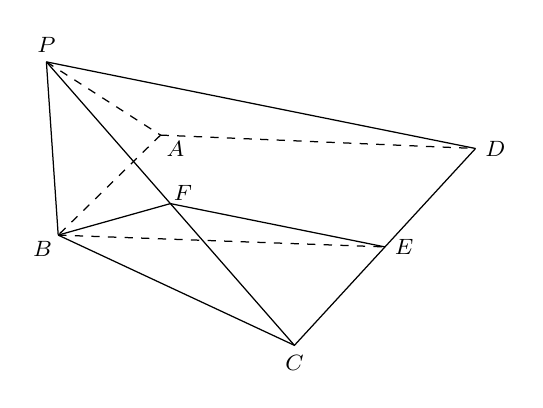
\begin{tikzpicture}[font=\footnotesize, line width=0.45pt]
  \coordinate (P) at (1.40,3.85);
  \coordinate (A) at (2.85,2.92);
  \coordinate (B) at (1.55,1.65);
  \coordinate (C) at (4.55,0.25);
  \coordinate (D) at (6.85,2.75);
  \coordinate (E) at (5.70,1.50);
  \coordinate (F) at (2.975,2.05);
  % 可见棱
  \draw (P) -- (B);
  \draw (P) -- (C);
  \draw (P) -- (D);
  \draw (B) -- (C) -- (D);
  \draw (B) -- (F) -- (E);
  % 被遮挡的棱
  \draw[dashed] (P) -- (A);
  \draw[dashed] (A) -- (B);
  \draw[dashed] (A) -- (D);
  \draw[dashed] (B) -- (E);
  % 顶点标注
  \node[above] at (P) {$P$};
  \node[below right, inner sep=2pt] at (A) {$A$};
  \node[below left, inner sep=2pt] at (B) {$B$};
  \node[below] at (C) {$C$};
  \node[right] at (D) {$D$};
  \node[right] at (E) {$E$};
  \node[above right, inner sep=1pt] at (F) {$F$};
\end{tikzpicture}
\end{center}
\nopagebreak[4]
\Needspace{4\baselineskip}
\textbf{解析}
\Needspace{5\baselineskip}
\textbf{（1）} 因为平面 $PAD\perp$ 底面 $ABCD$，且两平面交于 $AD$；又 $PA\subset$ 平面 $PAD$，$PA\perp AD$，由面面垂直的性质定理得
\nopagebreak[4]
\[PA\perp\text{\text{底面} }ABCD.\]

\Needspace{5\baselineskip}
\textbf{（2）} 因为 $AB\parallel CD$，$E$ 是 $CD$ 的中点，所以
\nopagebreak[4]
\[AB\parallel DE,\qquad AB=\frac12CD=DE,\]
\Needspace{5\baselineskip}
故四边形 $ABED$ 是平行四边形，从而
\nopagebreak[4]
\[BE\parallel AD.\]
\Needspace{5\baselineskip}
又 $AD\subset$ 平面 $PAD$，$BE\not\subset$ 平面 $PAD$，由线面平行的判定定理得
\nopagebreak[4]
\[BE\parallel\text{\text{平面} }PAD.\]

\Needspace{5\baselineskip}
\textbf{（3）} 在 $\triangle PCD$ 中，$E$，$F$ 分别是 $CD$，$PC$ 的中点，由中位线定理得
\nopagebreak[4]
\[EF\parallel PD.\]
\Needspace{5\baselineskip}
结合（2）中的 $BE\parallel AD$，且 $BE\cap EF=E$，$AD\cap PD=D$，得
\nopagebreak[4]
\[\text{\text{平面} }BEF\parallel\text{\text{平面} }PAD.\]
\Needspace{5\baselineskip}
另一方面，由 $AB\parallel CD$ 及 $AB\perp AD$ 得 $CD\perp AD$；由（1）$PA\perp$ 底面 $ABCD$ 及 $CD\subset$ 底面 $ABCD$ 得 $CD\perp PA$。于是 $CD\perp$ 平面 $PAD$，而 $CD\subset$ 平面 $PCD$，故
\nopagebreak[4]
\[\text{\text{平面} }PCD\perp\text{\text{平面} }PAD.\]
\Needspace{5\baselineskip}
再由平面 $BEF\parallel$ 平面 $PAD$ 得
\nopagebreak[4]
\[\text{\text{平面} }BEF\perp\text{\text{平面} }PCD.\]

\gkanswer{答案（1）：证明见解析。由面面垂直的性质，$PA\subset$ 平面 $PAD$ 且 $PA\perp$ 交线 $AD$，故 $PA\perp$ 底面 $ABCD$。}

\gkanswer{答案（2）：证明见解析。由 $AB\parallel DE$ 且 $AB=DE$ 得 $ABED$ 为平行四边形，故 $BE\parallel AD$；又 $AD\subset$ 平面 $PAD$，$BE\not\subset$ 平面 $PAD$，所以 $BE\parallel$ 平面 $PAD$。}

\gkanswer{答案（3）：证明见解析。$BE\parallel AD$，$EF\parallel PD$，故平面 $BEF\parallel$ 平面 $PAD$，而 $CD\perp$ 平面 $PAD$ 给出平面 $PCD\perp$ 平面 $PAD$。}

\end{answer}
\begin{answer}
\gksolhead{18}{}

\textbf{题目}：

已知函数 $f(x)=x^2+x\sin x+\cos x$。

（1） 若曲线 $y=f(x)$ 在点 $(a,f(a))$ 处与直线 $y=b$ 相切，求 $a$ 与 $b$ 的值；

（2） 若曲线 $y=f(x)$ 与直线 $y=b$ 有两个不同交点，求 $b$ 的取值范围。

\Needspace{4\baselineskip}
\textbf{解析}
\Needspace{5\baselineskip}
\textbf{（1）} 求导：
\nopagebreak[4]
\[f'(x)=2x+\sin x+x\cos x-\sin x=x(2+\cos x).\]
\Needspace{5\baselineskip}
曲线在点 $(a,f(a))$ 处与水平直线 $y=b$ 相切，切线斜率为 $0$，即
\nopagebreak[4]
\[f'(a)=a(2+\cos a)=0.\]
\Needspace{5\baselineskip}
因为 $2+\cos a\geqslant1>0$，所以只能 $a=0$，此时
\nopagebreak[4]
\[b=f(0)=0+0+1=1.\]
\Needspace{5\baselineskip}
故
\nopagebreak[4]
\[a=0,\qquad b=1.\]

\Needspace{5\baselineskip}
\textbf{（2）} 由（1），$f'(x)=x(2+\cos x)$，而 $2+\cos x>0$ 恒成立，故 $f'(x)$ 与 $x$ 同号：$f$ 在 $(-\infty,0)$ 上单调递减，在 $(0,+\infty)$ 上单调递增，在 $x=0$ 处取最小值
\nopagebreak[4]
\[f(0)=1.\]
又当 $x\to\pm\infty$ 时 $x^2$ 起主导作用，$f(x)\to+\infty$。因此：
当 $b<1$ 时，$f(x)\geqslant1>b$，无交点；
当 $b=1$ 时，只有 $x=0$ 一个交点；
当 $b>1$ 时，$(-\infty,0)$ 与 $(0,+\infty)$ 上各恰有一个交点，共两个不同交点。
\Needspace{5\baselineskip}
故
\nopagebreak[4]
\[b\in(1,+\infty).\]

\gkanswer{答案（1）：$a=0$，$b=1$。$f'(x)=x(2+\cos x)$，切线水平要求 $f'(a)=0$，得 $a=0$，$b=f(0)=1$。}

\gkanswer{答案（2）：$(1,+\infty)$。$f$ 在 $x=0$ 处取最小值 $1$，且向两侧无界增大，故 $b>1$ 时恰有两个交点。}

\end{answer}
\begin{answer}
\gksolhead{19}{}

\textbf{题目}：

直线 $y=kx+m$（$m\neq0$）与椭圆 $W:\dfrac{x^2}4+y^2=1$ 相交于 $A$，$C$ 两点，$O$ 是坐标原点。

（1） 当点 $B$ 的坐标为 $(0,1)$，且四边形 $OABC$ 为菱形时，求 $AC$ 的长；

（2） 当点 $B$ 在 $W$ 上且不是 $W$ 的顶点时，证明：四边形 $OABC$ 不可能为菱形。

\Needspace{4\baselineskip}
\textbf{解析}
\Needspace{5\baselineskip}
\textbf{（1）} 四边形 $OABC$ 为菱形时，它也是平行四边形，对角线 $OB$ 与 $AC$ 互相垂直平分。由 $O(0,0)$，$B(0,1)$ 得 $OB$ 的中点
\nopagebreak[4]
\[M\left(0,\frac12\right),\]
\Needspace{5\baselineskip}
且 $OB$ 在 $y$ 轴上，故 $AC\perp OB$ 表明 $AC$ 是水平直线，即
\nopagebreak[4]
\[AC:\ y=\frac12.\]
\Needspace{5\baselineskip}
代入椭圆 $W:\dfrac{x^2}4+y^2=1$：
\nopagebreak[4]
\[\frac{x^2}4+\frac14=1\iff x^2=3\iff x=\pm\sqrt3.\]
\Needspace{5\baselineskip}
于是 $A$，$C$ 的横坐标之差为 $2\sqrt3$，即
\nopagebreak[4]
\[|AC|=2\sqrt3.\]
（此时 $|OA|=\sqrt{3+\dfrac14}=\dfrac{\sqrt{13}}2=|AB|$，确为菱形。）

\Needspace{5\baselineskip}
\textbf{（2）} 设 $B(x_0,y_0)$ 在 $W$ 上，即
\nopagebreak[4]
\[\frac{x_0^2}4+y_0^2=1.\]
\Needspace{5\baselineskip}
若 $OABC$ 为菱形，则它是平行四边形，且四边相等，于是
\nopagebreak[4]
\[|OA|=|AB|,\qquad |OC|=|CB|.\]
\Needspace{5\baselineskip}
设 $A(x_1,y_1)$，$C(x_2,y_2)$。由 $|OA|^2=|AB|^2$ 得
\nopagebreak[4]
\[x_1^2+y_1^2=(x_1-x_0)^2+(y_1-y_0)^2,\]
\Needspace{5\baselineskip}
化简得
\nopagebreak[4]
\[2x_0x_1+2y_0y_1=x_0^2+y_0^2.\]
\Needspace{5\baselineskip}
同理由 $|OC|^2=|CB|^2$ 得
\nopagebreak[4]
\[2x_0x_2+2y_0y_2=x_0^2+y_0^2.\]
\Needspace{5\baselineskip}
两式相减：
\nopagebreak[4]
\[x_0(x_1-x_2)+y_0(y_1-y_2)=0.\tag{1}\]
\Needspace{5\baselineskip}
又 $OABC$ 为平行四边形，故 $OB$ 与 $AC$ 互相平分，即
\nopagebreak[4]
\[x_1+x_2=x_0,\qquad y_1+y_2=y_0.\]
\Needspace{5\baselineskip}
而 $A$，$C$ 都在 $W$ 上，两式相减得
\nopagebreak[4]
\[\frac{x_1^2-x_2^2}4+(y_1^2-y_2^2)=0,\]
\Needspace{5\baselineskip}
即
\nopagebreak[4]
\[\frac{(x_1-x_2)(x_1+x_2)}4+(y_1-y_2)(y_1+y_2)=0,\]
\Needspace{5\baselineskip}
代入 $x_1+x_2=x_0$，$y_1+y_2=y_0$ 得
\nopagebreak[4]
\[\frac{x_0(x_1-x_2)}4+y_0(y_1-y_2)=0.\tag{2}\]
\Needspace{5\baselineskip}
由（1）（2）消去 $y_0(y_1-y_2)$：将（1）减去（2）得
\nopagebreak[4]
\[\frac34x_0(x_1-x_2)=0.\]
若 $x_0=0$，则 $B(0,\pm1)$ 是 $W$ 的顶点，与题设矛盾；故 $x_1=x_2$。代回（1）得 $y_0(y_1-y_2)=0$，而 $y_0\neq0$（否则 $B(\pm2,0)$ 也是顶点），故 $y_1=y_2$。于是 $A=C$，与 $AC$ 是对角线矛盾。

所以四边形 $OABC$ 不可能为菱形。

\gkanswer{答案（1）：$2\sqrt3$。菱形对角线互相垂直平分，$AC$ 为 $y=\dfrac12$ 被椭圆截得的弦。}

\gkanswer{答案（2）：证明见解析。若为菱形则由 $|OA|=|AB|$、$|OC|=|CB|$ 与 $A$，$C$ 在 $W$ 上推出 $x_0y_0=0$，与 $B$ 不是顶点矛盾。}

\end{answer}
\begin{answer}
\gksolhead{20}{}

\textbf{题目}：

给定数列 $a_1$，$a_2$，$\cdots$，$a_n$，对 $i=1$，$2$，$\cdots$，$n-1$，该数列前 $i$ 项的最大值记为 $A_i$，后 $n-i$ 项 $a_{i+1}$，$a_{i+2}$，$\cdots$，$a_n$ 的最小值记为 $B_i$，$d_i=A_i-B_i$。

（1） 设数列 $\{a_n\}$ 为 $3$，$4$，$7$，$1$，写出 $d_1$，$d_2$，$d_3$ 的值；

（2） 设 $a_1$，$a_2$，$\cdots$，$a_n$（$n\geqslant4$）是公比大于 $1$ 的等比数列，且 $a_1>0$。证明：$d_1$，$d_2$，$\cdots$，$d_{n-1}$ 是等比数列；

（3） 设 $d_1$，$d_2$，$\cdots$，$d_{n-1}$ 是公差大于 $0$ 的等差数列，且 $d_1>0$。证明：$a_1$，$a_2$，$\cdots$，$a_{n-1}$ 是等差数列。

\Needspace{4\baselineskip}
\textbf{解析}
\Needspace{5\baselineskip}
\textbf{（1）} 对数列 $3$，$4$，$7$，$1$：
\nopagebreak[4]
\[A_1=3,\quad A_2=\max\{3,4\}=4,\quad A_3=\max\{3,4,7\}=7,\]
\nopagebreak[4]
\[B_1=\min\{4,7,1\}=1,\quad B_2=\min\{7,1\}=1,\quad B_3=1.\]
\Needspace{5\baselineskip}
故
\nopagebreak[4]
\[d_1=3-1=2,\qquad d_2=4-1=3,\qquad d_3=7-1=6.\]

\Needspace{5\baselineskip}
\textbf{（2）} 设 $a_i=a_1q^{i-1}$，$q>1$，$a_1>0$，则 $a_1<a_2<\cdots<a_n$。于是前 $i$ 项的最大值就是第 $i$ 项，后 $n-i$ 项的最小值就是第 $i+1$ 项：
\nopagebreak[4]
\[A_i=a_i,\qquad B_i=a_{i+1}\quad(i=1,2,\cdots,n-1).\]
\Needspace{5\baselineskip}
所以
\nopagebreak[4]
\[d_i=a_i-a_{i+1}=a_1q^{i-1}-a_1q^{i}=a_1(1-q)q^{i-1}.\]
\Needspace{5\baselineskip}
因为 $q>1$，$a_1>0$，故 $a_1(1-q)\neq0$，$d_i\neq0$；且对 $i=1,2,\cdots,n-2$，
\nopagebreak[4]
\[\frac{d_{i+1}}{d_i}=\frac{a_1(1-q)q^{i}}{a_1(1-q)q^{i-1}}=q,\]
比值为非零常数。所以 $d_1$，$d_2$，$\cdots$，$d_{n-1}$ 是公比为 $q$ 的等比数列。

\Needspace{5\baselineskip}
\textbf{（3）} 设等差数列 $d_1$，$d_2$，$\cdots$，$d_{n-1}$ 的公差为 $D>0$（$n\leqslant2$ 时结论显然，以下设 $n\geqslant3$），则
\nopagebreak[4]
\[d_{i+1}-d_i=D>0\quad(i=1,2,\cdots,n-2).\]
\Needspace{5\baselineskip}
由 $A_{i+1}=\max\{A_i,a_{i+1}\}\geqslant A_i$ 及 $B_i=\min\{a_{i+1},B_{i+1}\}\leqslant B_{i+1}$，有
\nopagebreak[4]
\[d_{i+1}-d_i=(A_{i+1}-A_i)+(B_i-B_{i+1})\leqslant A_{i+1}-A_i.\]
\Needspace{5\baselineskip}
而左端等于 $D>0$，故 $A_{i+1}>A_i$，即 $a_{i+1}>A_i$ 对 $i=1,2,\cdots,n-2$ 成立。于是
\nopagebreak[4]
\[a_1<a_2<\cdots<a_{n-1},\qquad A_i=a_i\quad(i=1,2,\cdots,n-1).\]

\Needspace{5\baselineskip}
再由 $d_1=a_1-B_1>0$，其中 $B_1=\min\{a_2,a_3,\cdots,a_n\}$。因为 $a_2,\cdots,a_{n-1}$ 都严格大于 $a_1$，若 $a_n\geqslant a_1$ 则 $B_1\geqslant a_1$，从而 $d_1=a_1-B_1\leqslant0$，与 $d_1>0$ 矛盾，故 $a_n<a_1$，且
\nopagebreak[4]
\[B_1=a_n.\]
\Needspace{5\baselineskip}
由于 $a_{i+1},\cdots,a_{n-1}$ 都大于 $a_1>a_n$，对每个 $i=1,2,\cdots,n-1$ 都有
\nopagebreak[4]
\[B_i=\min\{a_{i+1},\cdots,a_n\}=a_n.\]
\Needspace{5\baselineskip}
因此
\nopagebreak[4]
\[d_i=A_i-B_i=a_i-a_n\quad(i=1,2,\cdots,n-1),\]
\Needspace{5\baselineskip}
从而对 $i=1,2,\cdots,n-2$，
\nopagebreak[4]
\[a_{i+1}-a_i=d_{i+1}-d_i=D.\]
即 $a_1$，$a_2$，$\cdots$，$a_{n-1}$ 是公差为 $D$ 的等差数列。

\gkanswer{答案（1）：$d_1=2$，$d_2=3$，$d_3=6$。$A_1=3$，$A_2=4$，$A_3=7$，而 $B_1=B_2=B_3=1$。}

\gkanswer{答案（2）：证明见解析。数列递增，$A_i=a_i$，$B_i=a_{i+1}$，故 $d_i=a_1(1-q)q^{i-1}$ 是公比为 $q$ 的等比数列。}

\gkanswer{答案（3）：证明见解析。由 $d_i$ 递增得 $a_2<\cdots<a_{n-1}$ 且 $a_n$ 为最小项，从而 $B_i=a_n$，$d_i=a_i-a_n$ 为等差数列。}

\end{answer}